\documentclass[12pt]{article}
\usepackage{mathptmx}
%\usepackage{kantlipsum}
\usepackage[margin=1in]{geometry}
\usepackage{setspace}
\usepackage{graphicx}



\title{Detecting ``Fake News" on Facebook}
\author{Hannah Eyre \and Zane Zakraisek}
\begin{document}
\maketitle
\setstretch{1.2}

The term ``Fake News" gained popularity during the United States' 2016 Presidential Election to describe a rapidly spreading phenomena of news articles deliberately spreading false information and hoaxes, often through attention grabbing headlines or headlines that resemble legitimate sources \cite{guardian}. It became particularly notorious on social media sites and Facebook in particular, where the top 20 articles from hoax sites and hyperpartisan blogs garnered more user interaction between August 1st and election day on November 8th than the top 20 articles from a variety of established news sources such as {\it The New York Times}, {\it Washington Post}, {\it Business Insider}, and Fox News \cite{buzzfeed}.

FactCheck.org, part of the Annberg Public Policy Center at the University of Pennsylvania, breaks down how an individual can identify fake news into eight parts \cite{factcheck}:
\begin{enumerate}
\item Consider whether the source is credible.
\item Read beyond the headline.
\item Check whether the author is credible or real.
\item Check whether the article is recent.
\item Check whether it is a joke or satire.
\item Consider your own biases and how they affect your judgment.
\item Check supporting sources (if any) and make sure they abide by the same rules.
\item Ask experts or fact-checking sites.
\end{enumerate}

Rapidly spreading fake news articles have a range of consequences, one instance culminating in a gunman attacking a Washington, DC pizza parlor over allegations of child pornography and child sex abuse ring centered around John Podesta, Hillary Clinton's 2016 campaign manager, in a conspiracy called ``Pizzagate" \cite{pizzagate}. Various politicians and government agencies in the United States and internationally have voiced opinions on what qualifies as fake news and what do do about it, but no consensus has been reached. Facebook was initially reluctant to admit there was any problem with fake news on news feeds, however Facebook's CEO Mark Zuckerberg has since released a statement describing how they plan to deal with fake news in the future, including renaming the phenomenon ``false news" \cite{zuckerberg}.

As an increasingly global and hotly contested issue, we would like to to explore what responsibility Facebook has in regards to these eight points. We will discuss whether they have a responsibility to develop tools to detect fake news based off these guidelines and, if these tools exist, whether they should be used to remove content from the site.

When analyzing any issue, it's important to define what framework you're working in, along with what premisses your arguments are based on. During our analyzation of the Facebook's role in censorship, we'll be working under a utilitarian framework. In particular, we'll be using a utilitarian framework designed to minimize the harm. We have chosen this particular form of utilitarianism for a few different reasons. If you examine the role that fake news has played in the numerous events mentioned, it's evident that the outcome is negative in a large majority of occurrences. It's true that news in general on Facebook has the potential to result in positive utility among its readers, but as we've seen, more often than not the potential negatives don't come close to outweighing the corresponding positives. As a result, while it's important to attempt to maintain the positive utility brought about by Facebook's news feeds, we believe that it's far more important to try to minimize the corresponding negative utility.

As we address each of these eight points, the format shall be as follows. We'll first examine the outcome if Facebook chose not to implement this fake news filtering mechanism. Next, we'll examine the outcome if Facebook chose to implement the mechanism. Lastly, we'll weigh the different utilities and select the one that we feel minimizes the negative utility. In addition to this, we'll also be examining whether or not the method is even technically feasible to implement. The final outcome for each point will be a combination of the two points. 



\section{Credible sources: Sites and Authors}
The first method in combatting the spreading of fake news is to check whether the article in question comes from a credible source. This involves not just the author, the site itself. To start off, we'll examine the utility if Facebook chose \textit{not to} implement this source credibility check. Although Facebook currently implements a very light form of censorship (CITE), the scenario would be quite similar to how Facebook currently monitors articles, which is very little. While most articles that Facebook feeds users are based off of topics that they've shown interest in, nearly every Facebook user has probably been shown an article from an underground website that someone on their friends list has liked or shared. If Facebook didn't implement source credibility prioritization, then the effect of one person sharing an article like this could have quite a negative outcome. The article in question can easily make its way to hundreds of people. For most fake news articles, this has the effect of increasing the amount of negative utility, as most fake news articles are spread with negative motives.

Now assume Facebook was to implement source credibility prioritization. In this same scenario, if someone was to like or share a post, Facebook could first check its feedback for that particular site and/or author. If there is enough feedback, and the score is negative, Facebook could deprioritize the article on other people's news feeds by a factor of the magnitude of the negative score. Likewise, if the site or author has a positive score, Facebook could choose to display the article as it normally would, or maybe even prioritize it higher. From a utility perspective, this has the potential to significantly reduce negative utility brought about by fake cites. On the other hand, there does exist the potential to filter out some cites which many people may find to be \textit{good}. In other words, this has the potential to significantly decrease negative utility, with a smaller side effect of decreasing some positive utility. From an overall perspective however, implementing source credibility prioritization has the net effect of decreasing negative utility

In terms of the technical feasibility of this point, we feel like it one of the lowest hanging fruit in the pursuit of diminishing fake news. Once possibility would involve Facebook storing a few metrics for a site based upon feedback received by readers. Facebook already has a way to flag particular articles as inappropriate. In the same way, Facebook could allow a reader to optionally rate the credibility of the article or the site in general, and use these ratings to prioritize and deprioritize sites. 

Lastly, there's the idea of checking whether or not the author of an article is indeed a real person, and is indeed who they claim to be. We feel that this would be a much more difficult task for Facebook to implement. Additionally, while author authentication is a concept that would indeed help lower negative utility, the implementation of it would most likely cross the privacy line. This in turn increases negative utility. For example, Facebook may attempt to link the author of an article on some site to an individual account on Facebook for an added level of author verification. Since this has implications in terms of privacy, we feel that author authentication is not an angle that Facebook should approach this problem from.



\section{Reading Beyond the Headline}
When posting an external link to Facebook, information is drawn from the content inside \texttt{meta} elements of the page source by Facebook's web crawler and placed into a preview on the post itself. If an element labeled according to the Open Graph protocol, the crawler will place it in the link preview on the site \cite{fbwebmaster}. With this system in place, every linked website will appear the same on a users news feed. Any site can determine how its posts show up when linked on Facebook, regardless of the quality of the content or site itself. \\

\begin{figure}[h]
	\begin{minipage}{0.48\textwidth}
		\centering
		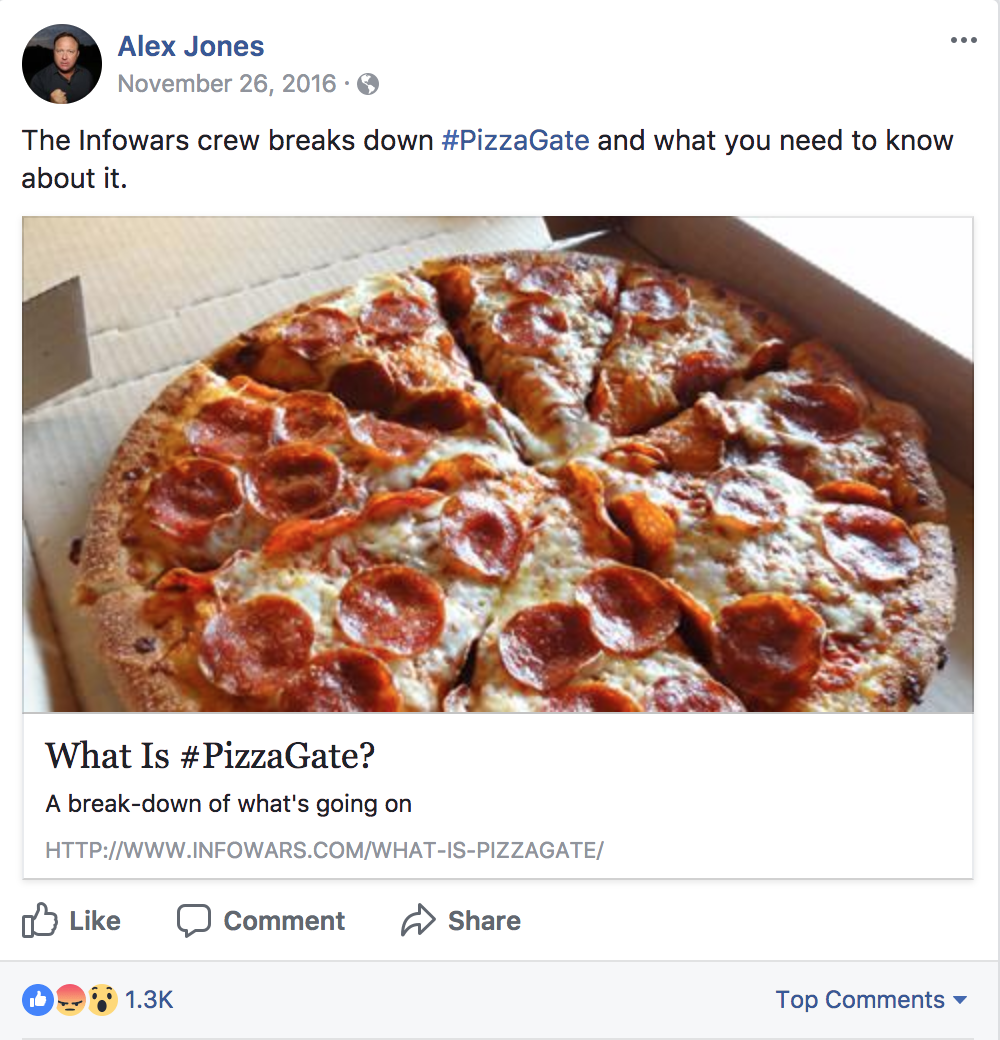
\includegraphics[scale=.3]{pizzagate_alex_jones_fb}
	\end{minipage}
	\begin{minipage}{0.48\textwidth}
		\centering
		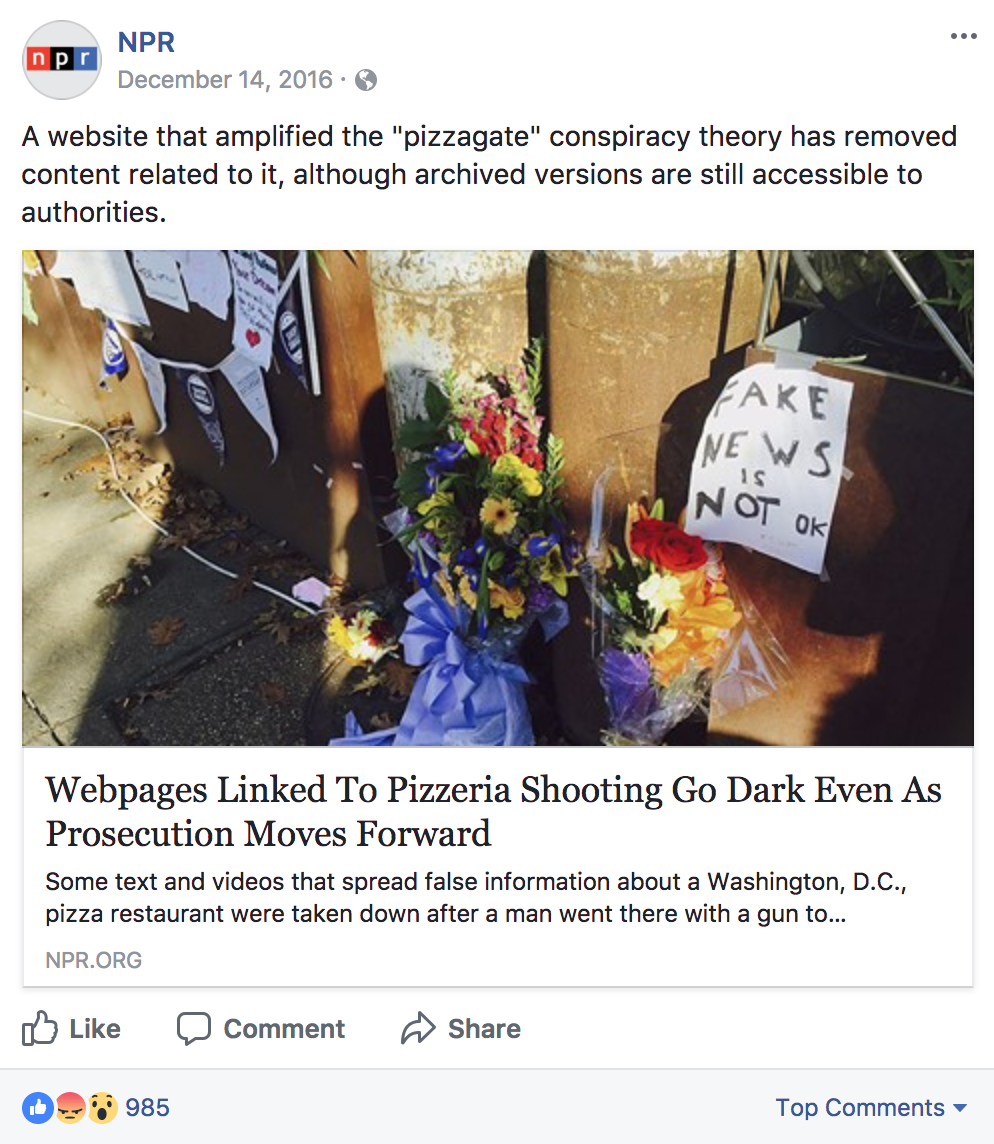
\includegraphics[scale=.3]{pizzagate_npr_fb}
	\end{minipage}
	\caption{A comparison of posts by Alex Jones, creator of {\it Infowars}, \cite{alex_jones_pizzagate_post} and {\it NPR} \cite{npr_pizzagate_post} about Pizzagate.}
\end{figure}

This uniform formatting treats {\it NPR} and {\it Infowars} or any other site that uses the \texttt{meta} elements according to Facebook's specifications as equals. It places less emphasis on the source of the article than on the headline and picture. The examples above are posted from official accounts, allowing users to easily see where the article comes from. However, the same articles posted by friends or unofficial pages make the source more difficult to determine.

In addition, because the information taken by the Facebook crawler is entirely determined by the web developer, the headline, picture, and description can be completely misleading.






\section{Age of the Article: Hannah}
Considering the age of the article is an important aspect of identifying fake news. Both very recent articles and older articles can be subject to scrutiny.

Manipulating trending topics with new, uninformed articles

quoting old sources with no date



\section{Article Genre: Hannah}

the onion, dedicated satire site, https://www.theonion.com/no-way-to-prevent-this-says-only-nation-where-this-r-1819580358

new yorker, sometime satire, 

"just a joke" defense for harassment, 



\section{Interpretation Bias: Hannah}

facebook demographics, http://journals.sagepub.com/doi/abs/10.1177/2053168017720008

trending topic staff fired, https://www.theguardian.com/technology/2016/aug/29/facebook-fires-trending-topics-team-algorithm



\section{Cross Reference: Zane}



\section{Supporting sources: Zane}
The final method for identifying fake news is to check supporting sources (if any) and make sure they abide by the same rules. In other words, this method attacks the problem with a recursive approach. When a user shares an article on the site, the fake news algorithm could take a depth first approach at calculating a trustworthiness metric. This can be done by first calculating the trustworthiest of the sources linked to in the article, and then using this metric in the overall trustworthiness calculation for the main article. 

From a utilitarian perspective where our main goal is to minimize the amount of negative utility brought about by fake articles, we feel that implementing this method has a few angles to consider. Since this method is basically taking the other methods that we feel are appropriate, and applying them in a recursive manner, we feel that for the most part this would be an extra step in minimizing the spread of fake news. One point to keep in mind however is that by taking a recursive approach, we may be rating the credibility of one page based on the credibility of a page with multiple degrees of separation that have virtually nothing to do with each other. Also, as mentioned in \textit{Credible Cites and Sources}, we don't have a way to flag a link with the context that it's being cited in. For example, if an author is citing a fake news article with the intention of pointing out the fake news, the trustworthiness metric should somehow understand this context, and not use this against the articles score.

In terms of the technical feasibility of the implementation, there are a few issues that would make this point difficult to implement. The first hurdle is that there would have to be some kind of standardization to the method that sites use to track citations and references. Most sites that people read have a nonstandard citations section at the bottom of the page. Although this conveys the required information to the \textit{reader}, it fails to be parsable by a web crawler. Additionally, this depth first approach to calculating source credibility would involve storing a large amount of metadata. LINK SHORTENERS


\paragraph{Final utility based on points above}

\newpage
\bibliographystyle{apalike}
\bibliography{proposal_bibliography.bib}


\end{document}
